\section{Method}
\label{sec:method}

\subsection{Problem}
Given an image or a video $I$ and a question $Q$, the encoder produces $N$ visual positions $\mathcal{V}$. The decoder has $L$ layers. Layer $\ell$ reads a visual set $S^{(\ell)}$. The visual token-layer budget and its layer average are
\begin{equation}
W=\sum_{\ell=1}^{L}|S^{(\ell)}|\le W_{\max},\qquad \bar K=W/L.
\label{eq:budget}
\end{equation}
$W$ counts visual positions seen by each layer. It is not FLOPs, latency, or memory. Let $S_0$ be a question-free basis of size $K$, $q_i$ a question score, and $C(S)$ a coverage of all original positions. Entry adaptation solves
\begin{equation}
\max_{S\subseteq\mathcal{V}}\sum_{i\in S} q_i
\quad\text{s.t.}\quad
|S|=K,\;
|S\triangle S_0|/2\le B,\;
C(S)\ge C(S_0)-\delta.
\label{eq:opt}
\end{equation}
$B$ bounds the number of identity edits and $\delta$ bounds coverage distortion. The implemented search does not claim a global optimum of Eq.~\eqref{eq:opt}. It builds $S_0$, then accepts a bounded number of one-for-one exchanges that stay inside a coverage envelope. The selected indices gather the original projected rows. Concrete capacities belong to the experimental schedule, not to this definition.

\subsection{Cross-depth descriptors}
Middle and deep features $F_i^{\mathrm{m}}$ and $F_i^{\mathrm{d}}$ share patch indices. $\hat f_i^{a}=F_i^{a}/\|F_i^{a}\|_2$, and $s_i^{a}$ is the sum of heads of CLS-to-patch attention. A shared weight $\beta\in(0,1)$ builds the selection descriptor and the fused salience,
\begin{equation}
z_i=\bigl[\sqrt{1-\beta}\,\hat f_i^{\mathrm{d}};\;\sqrt{\beta}\,\hat f_i^{\mathrm{m}}\bigr],
\quad
s_i=(1-\beta)s_i^{\mathrm{d}}+\beta s_i^{\mathrm{m}}.
\label{eq:dual}
\end{equation}
The inner product $z_i^{\top}z_j$ is a weighted sum of the two depth-wise cosines. $s_i$ sets the anchor order and $z_i$ measures local complementarity. $z_i$ is not the tensor sent to the language model.

\subsection{Regional quotas}
Anchors are the top $K-b$ positions by $s$. The residual pool is everything outside the top $K$, not the complement of the anchors:
\begin{equation}
H=\mathrm{Top}_{K-b}(s;\mathcal{V}),\qquad R=\mathcal{V}\setminus\mathrm{Top}_{K}(s;\mathcal{V}).
\label{eq:pools}
\end{equation}
The grid is split into disjoint regions $V_g$. A region that contains anchors uses their normalized descriptor sum as a prototype $p_g$. With $g(i)$ the region of position $i$,
\begin{equation}
c_i=z_i^{\top}p_{g(i)},\qquad
u_i=s_i\bigl[1-\mathrm{clip}(c_i,0,1)\bigr].
\label{eq:util}
\end{equation}
Only candidates with a valid prototype and $c_i>0$ enter the utility sort. Each region contributes at most $\tau$ of them. If the quota cannot fill $b$ seats, $\tau$ increases. Any remainder is filled by salience, preferring regions that already have anchors. The basis is $S_0=H\cup D$. The quota is a count on the same utility, not a second coverage objective.

\subsection{Coverage-constrained query-guided exchange}
\label{sec:qge}
\noindent\begin{minipage}{\linewidth}
\centering
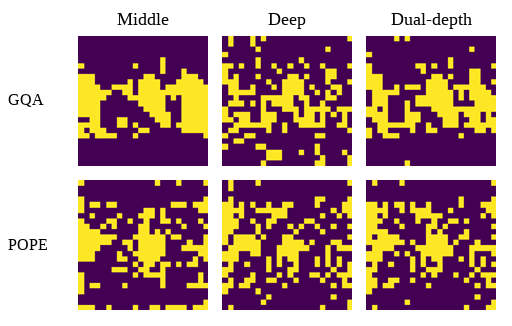
\includegraphics[width=\linewidth]{figures/depth_panels.png}
\captionof{figure}{Cross-depth selections at one kept count. Yellow cells are retained patches. GQA and POPE are centered on their rows. Middle selections form larger blocks. Deep selections are more scattered.}
\label{fig:depth}
\end{minipage}

Figure~\ref{fig:depth} is the same-capacity contrast behind the basis that QGE edits. Content words of the question, excluding options, instructions, and OCR lines, are averaged in the original embedding to $\bar e_Q$. For a native projected row $x_i$, the raw cosine is $a_i=\cos(x_i,\bar e_Q)$, and the question score is
\begin{equation}
q_i=\sigma\Bigl(\mathrm{clip}\bigl((a_i-\mathrm{med}(a))/(\kappa\,\mathrm{std}(a)),-c,c\bigr)\Bigr).
\label{eq:q}
\end{equation}
$G_{ij}$ is the mean over views of the cosine clipped to $[0,1]$. Coverage and novelty are
\begin{equation}
C(S)=N^{-1}\sum_{i\in\mathcal{V}}\max_{j\in S}G_{ij},\qquad
\nu(v\mid S)=1-\max_{j\in S}G_{vj}.
\label{eq:cov}
\end{equation}
Drop and donor priorities are $\pi^{-}_{u}=1-q_u+\lambda_r\max_{j\in S\setminus\{u\}}G_{uj}$ and $\pi^{+}_{v}=q_v\nu(v\mid S)$. For $S'=(S\setminus\{u\})\cup\{v\}$, write $\Delta q=q_v-q_u$ and $\Delta C=C(S')-C(S)$. A feasible pair needs $\Delta q\ge\gamma$, $\nu(v\mid S)\ge\eta$, and $\Delta C\ge-\varepsilon$. Each round then solves
\begin{equation}
\max_{u,v}\;\Delta q\,\nu(v\mid S)+\lambda_c\Delta C.
\label{eq:swap}
\end{equation}
The search stops when no pair passes the gates or $B$ exchanges have been accepted. The result $S_Q$ obeys
\begin{equation}
|S_Q\triangle S_0|/2\le B,\qquad C(S_Q)\ge C(S_0)-B\varepsilon.
\label{eq:env}
\end{equation}
Choosing $\delta\ge B\varepsilon$ places this envelope inside Eq.~\eqref{eq:opt}. The envelope bounds a feature proxy, not answer correctness.

\subsection{Question-to-visual attention refinement}
At cut $\ell_j$ the schedule asks for a nonincreasing size $K_j$, starting from $R_0=S_Q$. Q-Attn reads the question-token queries and the keys of the legal prefix under the model mask $M$,
\begin{equation}
A^{\ell_j,h}_{t,k}=\mathrm{softmax}_{k}\bigl((q^{\ell_j,h}_t)^{\top}k^{\ell_j,h}_k/\sqrt{d_h}+M_{t,k}\bigr).
\label{eq:attn}
\end{equation}
Let $p_j(i)$ be the current-sequence position of original index $i$. Summing over heads and question positions $\mathcal{T}_Q$ gives the keep score, and the next set is the top $K_j$ survivors of the previous set. Retained tokens keep their original position ids. If capacity $K_j$ lasts for $n_j$ layers, then $W=\sum_j n_j K_j$. The entry decides which evidence can participate. Each cut decides how far that evidence continues.
